\documentclass{beamer} % "Beamer" is a word used in Germany to mean video projector. 

\usetheme{Montpellier} % Search online for beamer themes to find your favorite or use the Berkeley theme as in this file.

\usecolortheme{rose}
\usepackage[utf8x]{inputenc}
\usepackage[english,russian]{babel}
\usepackage{color} % It may be necessary to set PCTeX or whatever program you are using to output a .pdf instead of a .dvi file in order to see color on your screen.
\usepackage{graphicx} % This package is needed if you wish to include external image files.

\usepackage{amsmath}
\usepackage{ulem}
\theoremstyle{definition} % See Lesson Three of the LaTeX Manual for more on this kind of "proclamation."
\newtheorem*{dfn}{A Reasonable Definition}               

\title{Оптимизация параметров стратегий поиска объектов на море}
\author{Антон Ковшаров} 
\institute{Санкт-Петербургский национальный исследовательский университет \\ информационных технологий, механики и оптики}
%\date{mm 15, 2015} 

\AtBeginSection[]  % The commands within the following {} will be executed at the start of each section.
{
\begin{frame} % Within each "frame" there will be one or more "slides."  
\frametitle{Содержание} % This is the title of the outline.
\tableofcontents[currentsection]  % This will display the table of contents and highlight the current section.
\end{frame}
} %  Do not include the preceding set of commands if you prefer not to have a recurring outline displayed during your presentation.

\begin{document}

\beamertemplatetransparentcoveredmedium
\begin{frame} 
\titlepage
\end{frame}

\section{Постановка задачи}
\begin{frame}
\begin{columns}
\column{.6\textwidth}
\includegraphics<+>[width=\textwidth]{pics/pic03-1.png}
\includegraphics<+>[width=\textwidth]{pics/pic03-2.png}
\includegraphics<+>[width=\textwidth]{pics/pic03-3.png}
\includegraphics<+->[width=\textwidth]{pics/pic03-4.png}
\column{.4\textwidth}
\setbeamercovered{dynamic}
\begin{itemize}
\item<.(-3)>{Начальное распределение}
  \begin{itemize}
     \item Нормальное распределение
     \item Равномерное распределиние
  \end{itemize}
\item<.(-2)-.(0)>{Эволюция распределения (диффузия)}
\end{itemize}
\end{columns}
\end{frame}

\begin{frame}
\begin{columns}
\column{.6\textwidth}
\includegraphics<+>[width=\textwidth]{pics/pic04-1.png}
\includegraphics<+>[width=\textwidth]{pics/pic04-2.png}
\includegraphics<+>[width=\textwidth]{pics/pic04-3.png}
\column{.4\textwidth}
\begin{itemize}
    \item<.(-2)-.(-1)>{Построение маршрута поиска объекта, основываясь на поле вероятности}
    \item<.(0)>{Симуляция прохождения маршрута}
\end{itemize}
\end{columns}
\end{frame}

\begin{frame}
  \frametitle{Стратегии поиска}
\begin{columns}

\column{.6\textwidth}
\includegraphics<2>[width=\textwidth]{pics/pic05-comb.png}
\includegraphics<3, 5->[width=\textwidth]{pics/pic05-parallel_tacks.png}
\includegraphics<4>[width=\textwidth]{pics/pic05-expand_box.png}
\column{.4\textwidth}
\setbeamercovered{dynamic}
\begin{itemize}
  \item<1> ``Заданный маршрут''
  \item<2> ``Гребенка''
  \item<3, 5-> ``Параллельное галсирование''
  \item<4> ``Расширяющийся квадрат''
\end{itemize}

\end{columns}
\end{frame}

\begin{frame}[t]
\only<1>{Распределение вероятности}
\only<2->{\sout{Распределение вероятности}\\}
\only<2->
{
Распределение частиц\\
\pause
\begin{itemize}
  \pause
\item частица - гипотеза положения объекта поиска
  \pause
\item перемещение частиц с течением времени
  \pause
\item сбор частиц средством поиска
  \pause
\item больше собранных частиц --- больше вероятность обнаружить объект
\end{itemize}
}
\end{frame}

\begin{frame}
  \frametitle{Входные данные}
\begin{itemize}
\item $t$ --- время поиска
\item $A_{t_0}$ --- матрица начального распределения
\item $f(A_t, \Delta t) = A_{t+\Delta t}$ --- функция изменения распределения
\item $geom$ --- геометрия района поиска
\item $p_0$ --- начальное положение средства поиска
\item $l$ --- прямая задающая направление галсирования
\item $v$ --- cкорость средства поиска
\item $B$ --- матрица вероятности обнаружения средством поиска (для простоты - обнаружение в круге радиуса $r$ с вероятностью 1)
\end{itemize}
\end{frame}

\begin{frame}
  \frametitle{Выходные данные}
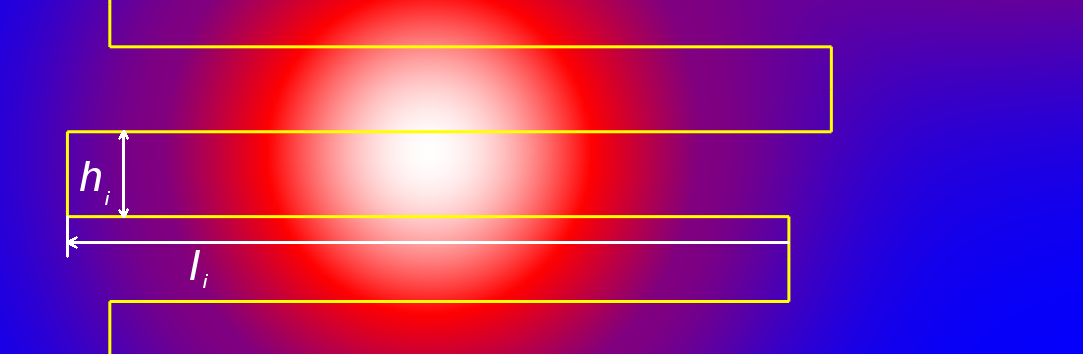
\includegraphics[width=\textwidth]{pics/pic06-lh.png}
\begin{itemize}
  \item $l_i$ --- проекция $i$-го галса на прямую $l$
  \item $h_i$ --- разница между галсом $i$ и $i+1$
  \item $S_{res}$ --- доля собранных частиц от начального распределения
\end{itemize}

\end{frame}

\begin{frame}
  \frametitle{Задача}
  Построить маршрут максимизирующий $S_{res}$
\end{frame}

\section{Симуляция эволюции распределения} % Since this is the start of a new section, our recurring outline will appear here.

\begin{frame} 
\frametitle{Диффузия}

Да, диффузия там взякая делается, все классно
\end{frame}

\section{Алгоритм построения маршрута}
\begin{frame}
\frametitle{Глобальный алгоритм}
Здесь нужно написать описание динамики за пятую степень
\end{frame}

\begin{frame}
\frametitle{Результаты работы глобального алгоритма}
\begin{columns}
\column{.6\textwidth}
\includegraphics<+>[width=\textwidth]{pics/pic01-clear.png}
\includegraphics<+>[width=\textwidth]{pics/pic01-1h.png}
\includegraphics<+>[width=\textwidth]{pics/pic01-2h.png}
\includegraphics<+>[width=\textwidth]{pics/pic01-3h.png}
\includegraphics<+>[width=\textwidth]{pics/pic01-4h.png}
\includegraphics<+>[width=\textwidth]{pics/pic01-8h.png}
\includegraphics<+->[width=\textwidth]{pics/pic01-16h.png}

\column{.4\textwidth}
\begin{itemize}
\setbeamercovered{dynamic}
\item<.(-6)>{исходное распределение}
\item<.(-5)>{1 час}
\item<.(-4)>{2 часa}
\item<.(-3)>{3 часa}
\item<.(-2)>{4 часa}
\item<.(-1)>{8 часов}
\item<.(0)>{16 часов}
\end{itemize}
\end{columns}
\end{frame}

\begin{frame}
\frametitle{Корректировка построенного пути}
\begin{columns}
\column{.6\textwidth}
\includegraphics<+>[width=\textwidth]{pics/pic02-init.png}
\includegraphics<+>[width=\textwidth]{pics/pic02-before.png}
\includegraphics<+>[width=\textwidth]{pics/pic02-after.png}

\column{.4\textwidth}
\begin{itemize}
\setbeamercovered{dynamic}
\item<.(-2)>{изначально построенный путь}
\item<.(-1)>{со временем путь устарел}
\item<.(0)>{перестроим путь}
\end{itemize}
\end{columns}

\end{frame}

\end{document}

%%% Local Variables:
%%% mode: latex
%%% TeX-master: t
%%% End:
